\documentclass{IOS-Book-Article}
\usepackage{mathptmx}
\usepackage{hyperref,url}
\usepackage{graphicx}
\usepackage{float}
\def\Eo{\mbox{\sc Ezo}}
\def\Ec{\mbox{\sc Ezo-CNN}}
\def\Ed{\mbox{\sc DeepEzo}}
\def\Mx{\mbox{\sc MoHex}}
\def\Mc{\mbox{\sc MoHex-CNN}}
\def\Mt{\mbox{\sc MoHex-3HNN}}
\def\Sol{\mbox{\sc Solver}}
\def\Fuego{\mbox{\sc Fuego}}

\def\hb{\hbox to 10.7 cm{}}

\begin{document}
\pagestyle{headings}
\def\thepage{}
\begin{frontmatter}              % The preamble begins here.
%\pretitle{Pretitle}
\title{Hex 2018: MoHex3HNN over DeepEzo}
\markboth{}{2018 New Taipei City Computer Olympiad Report: to appear in ICGA Journal}
\author{\fnms{Chao} \snm{Gao}} and
\author{\fnms{Kei} \snm{Takada}} and
\author{\fnms{Ryan} \snm{Hayward}\thanks{Corresponding 
  author: hayward@ualberta.ca.}}

\runningauthor{AuthorA et al.}
\address{Department of Computing Science, University of Alberta, Canada}
\end{frontmatter}
\markboth{Gao, Takada, Hayward}{\Mt\ defeats \Ed\ in Hex 2018}

\begin{figure}[hbt]
\includegraphics[width=\columnwidth]{photos/awards.eps}\
\caption{From left, Kei Takada, Chao Gao, Ryan Hayward}
\end{figure}
%convert hex-medallists.jpg -gravity Center -crop 95x66%+0+0 -compress lzw eps2:a.eps

\section{The Tournaments}
There were two Hex tournaments at the
2018 Computer Olympiad in New Taipei City:
11$\times$11 --- proposed by Piet Hein in 1942 ---
and 13$\times$13.\footnote{\cite{H18olyrptsource} has .sgf 
  game records and source files for this report.
  \cite{Hexgui} has an SGF (Smart Game Format) viewer.
  SGF was developed by \cite{SGF}.}

Visa problems unfortunately prevented Chinese teams from competing,
leaving two contestants for each tourament:
\Ed{} from Japan, by Kei Takada, supervised by Masahito Yamamoto;
and \Mt{} from Canada,
by Chao Gao, supervised by Ryan Hayward and Martin M\"{u}ller and
assisted by 
Jakub Pawlewicz,
Ashley Herman,
Joseph Meleshko,
Jiahao Li,
Paul Banse,
Siqi Yan,
Wai Yi Low
and
Xutong Zhao.
Gao and Pawlewicz developed a self-play game procedure,
used to select opening moves.

\Mt\ is an AlphaGo-style neural net program that shares code
with MoHex2.0 by 
Broderick Arneson, Philip Henderson, Aja Huang, 
Jakub Pawlewicz, Noah Weninger, Kenny Young and Ryan Hayward \cite{HAHMP13}.
MoHex versions have won the previous
eight Olympiad Hex competitions \cite{HW17}.
MoHex2.0 is an MCTS program that uses the Benzene Hex framework
built on the code base of \Fuego\ \cite{fuego}.

\Mt{}, the successor of \Mc,
uses a three-head convolutional neural net (CNN)
with 128 filters per layer \cite{GMH18}
trained on 400 000 self-play games.
At each new node of the Monte Carlo search tree, 
the three-headed neural net is called
and returns policy, state, and action values.
\Mt{} ran remotely on a machine with four CPU cores and one GPU.
Benzene's solver was not used:
all threads were used for tree computation.

%\Eo{}, based on the Benzene framework, 
%uses iterative deepening alpha-beta search 
%with policy and value functions
%learned from 10 000 000 self-play games
%generated by minimax search.
\Ed{} ran remotely on a machine
with two CPUs (one thread for search,
one for Benzene's solver) and one GPU.
In some games the internet connection dropped
and computation restarted on a laptop.

\Ed{}, written on the Benzene framework,
uses iterative deepening depth-first search and 
two CNN functions.
One is the evaluation function, which evaluates the current position.
The other is the policy function, 
which decides which moves to search next.
Moves whose value exceed a threshold are explored;
the rest are pruned.
Starting with random weights,
the two functions are built with reinforcement learning.
Learning games are generated by self-play with
depth-one minimax search.

On a 13$\times$13 board,
in a 676 game test
(all 1-move openings, 2 games as 1st player, 2 games as 2nd player),
with \Ed{} and MoHex2.0 allowed 30s/move and \Ec{}(2017) 
a 4-ply search,
\Ed{} wins about .80 and .85 of its games respectively against
MoHex2.0 and \Ec{}(2017).

The \Ed{} model for this competition had more
learning than the tested model, so might be even stronger.
2.6 million learning games were played.

{\bf Tournament results.}
Each tournament was best of 8 games,
with 30min/game per player.
The 13$\times$13 and 11$\times$11 tournaments were played
on July 8 and 9 respectively.
Each game ended by resignation as soon as an opponent win was detected.
\Mt\ won both tournaments 5-0.
See Figures~\ref{fig:13} and \ref{fig:11}.

\begin{figure}
\noindent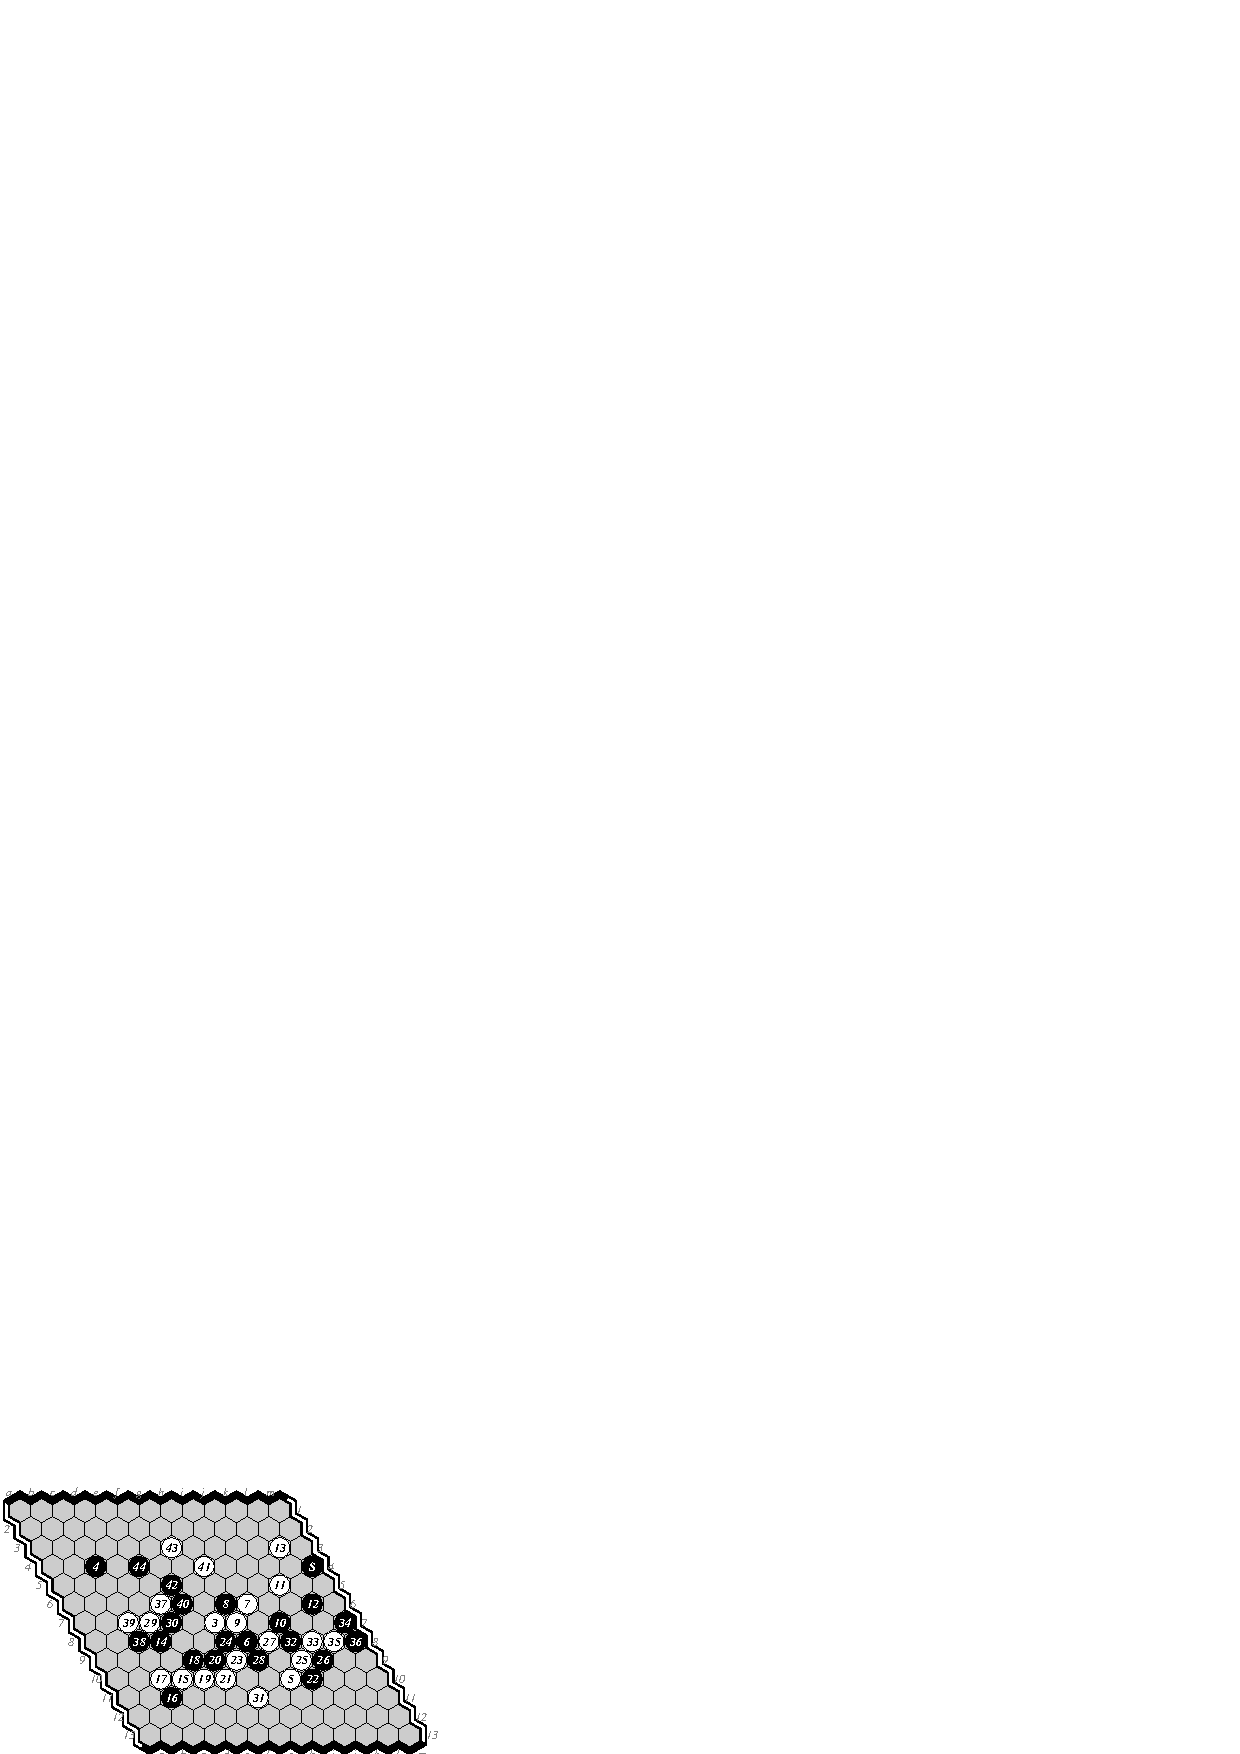
\includegraphics[width=.58\columnwidth]{pix/01-e-m}\hspace*{-.14\columnwidth}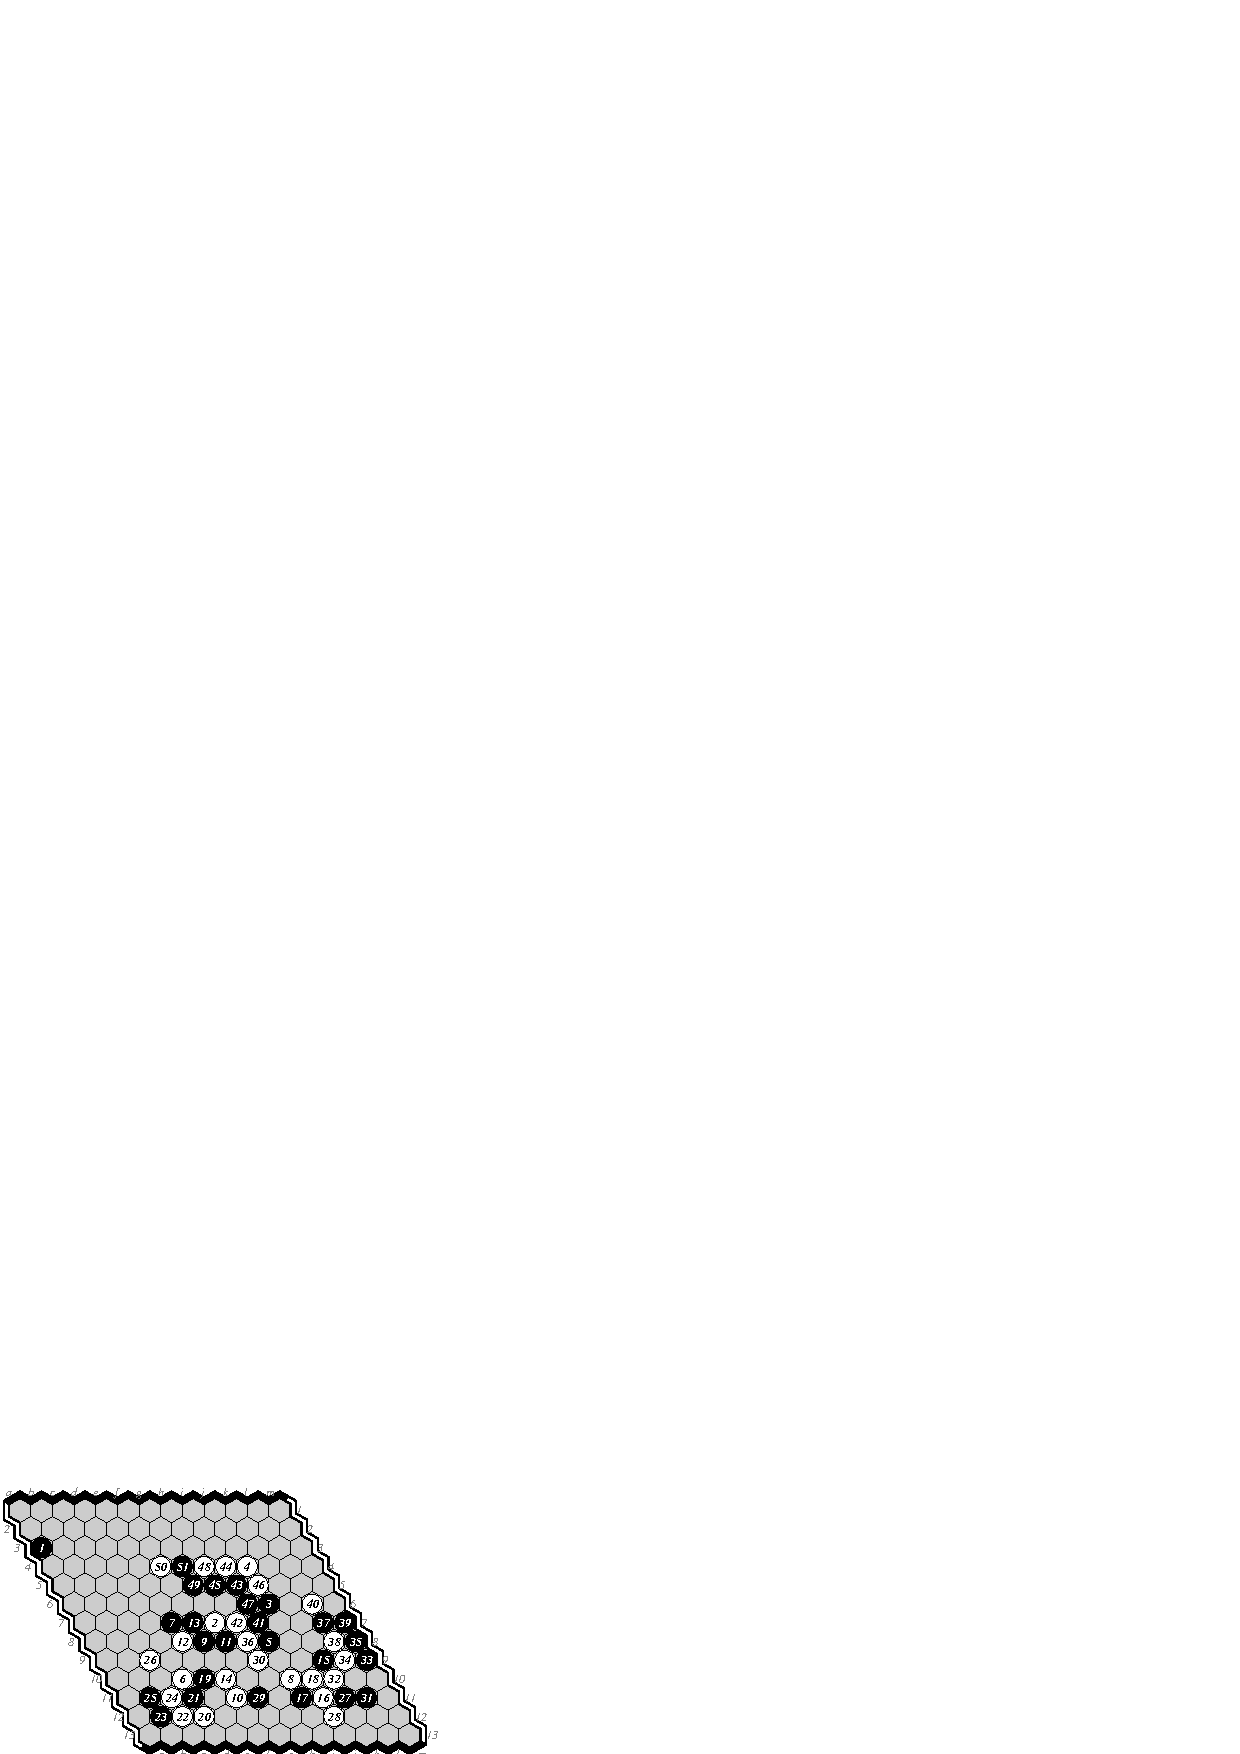
\includegraphics[width=.58\columnwidth]{pix/02-m-e}
\vspace*{.2cm}

\noindent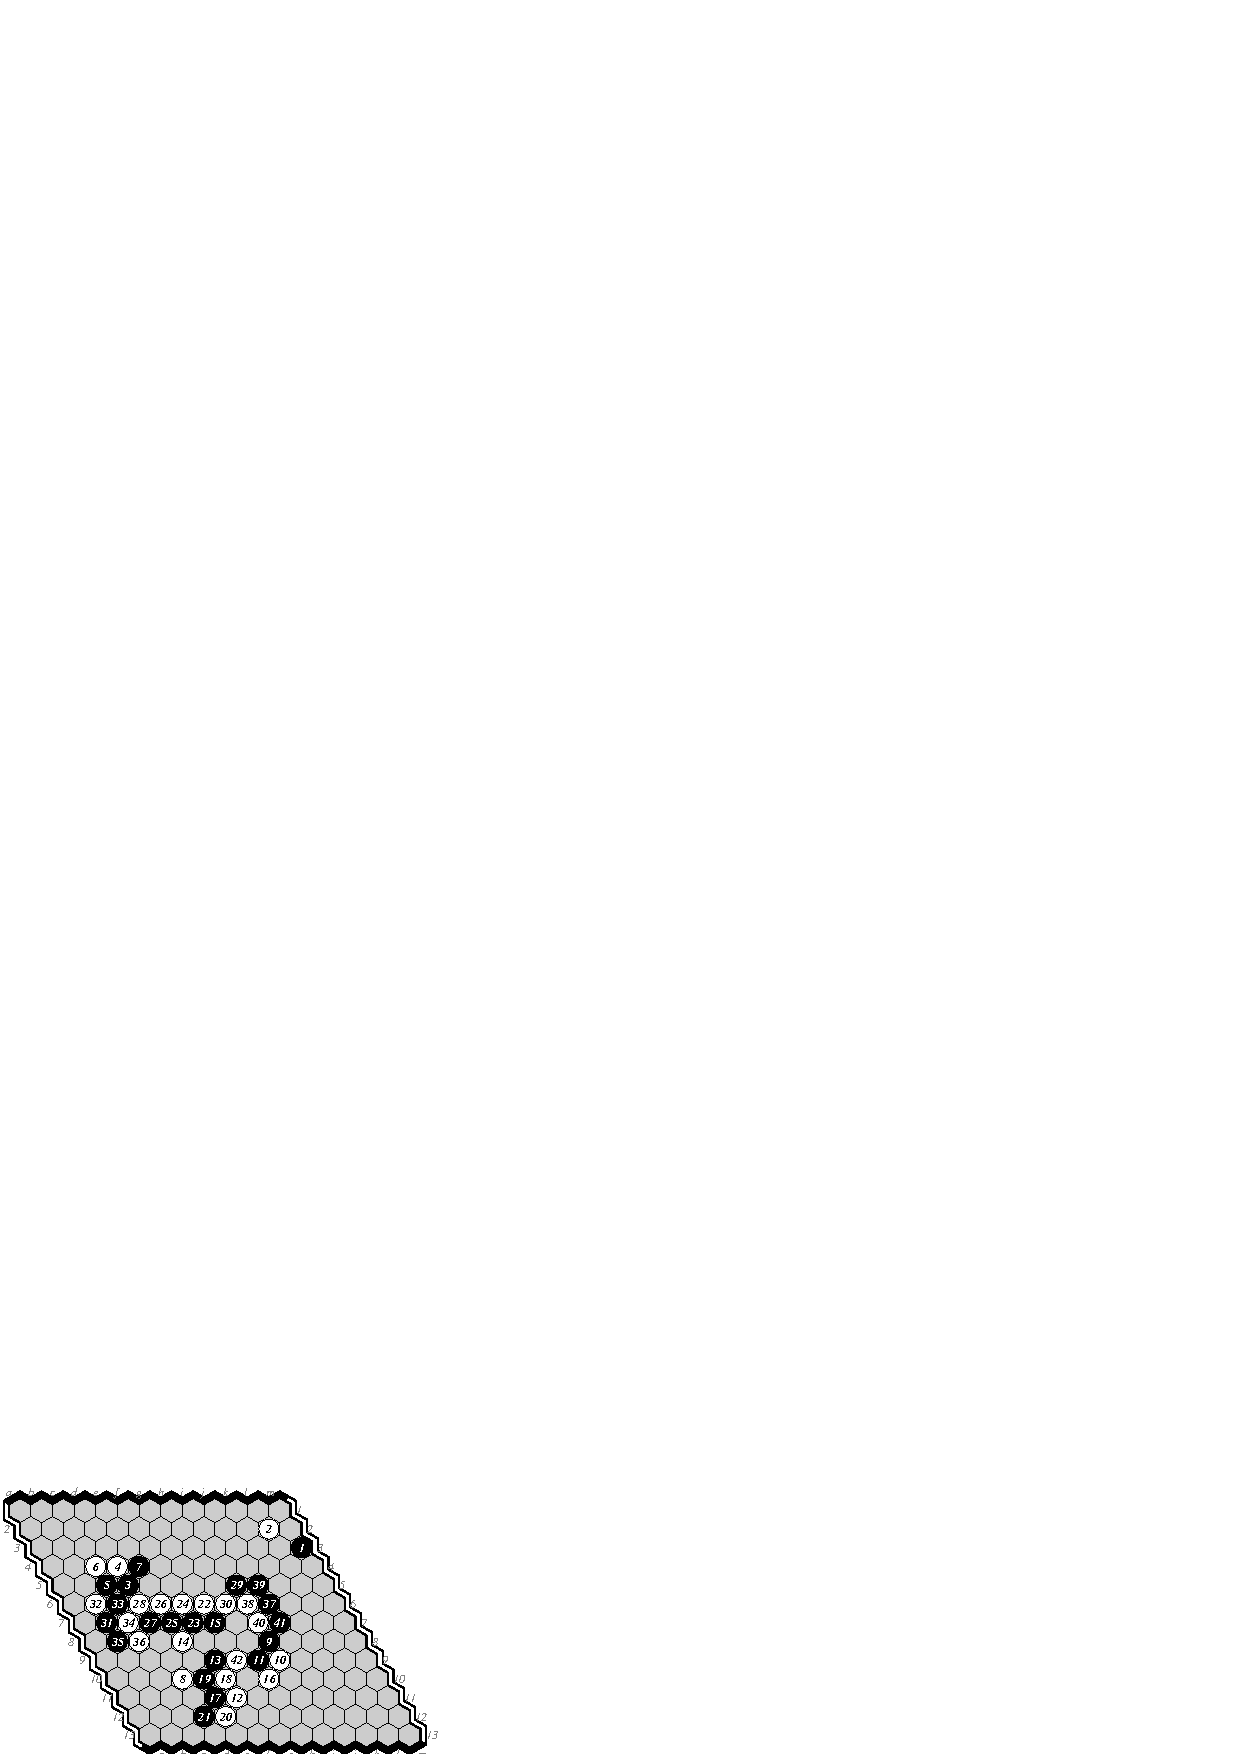
\includegraphics[width=.58\columnwidth]{pix/03-e-m}\hspace*{-.14\columnwidth}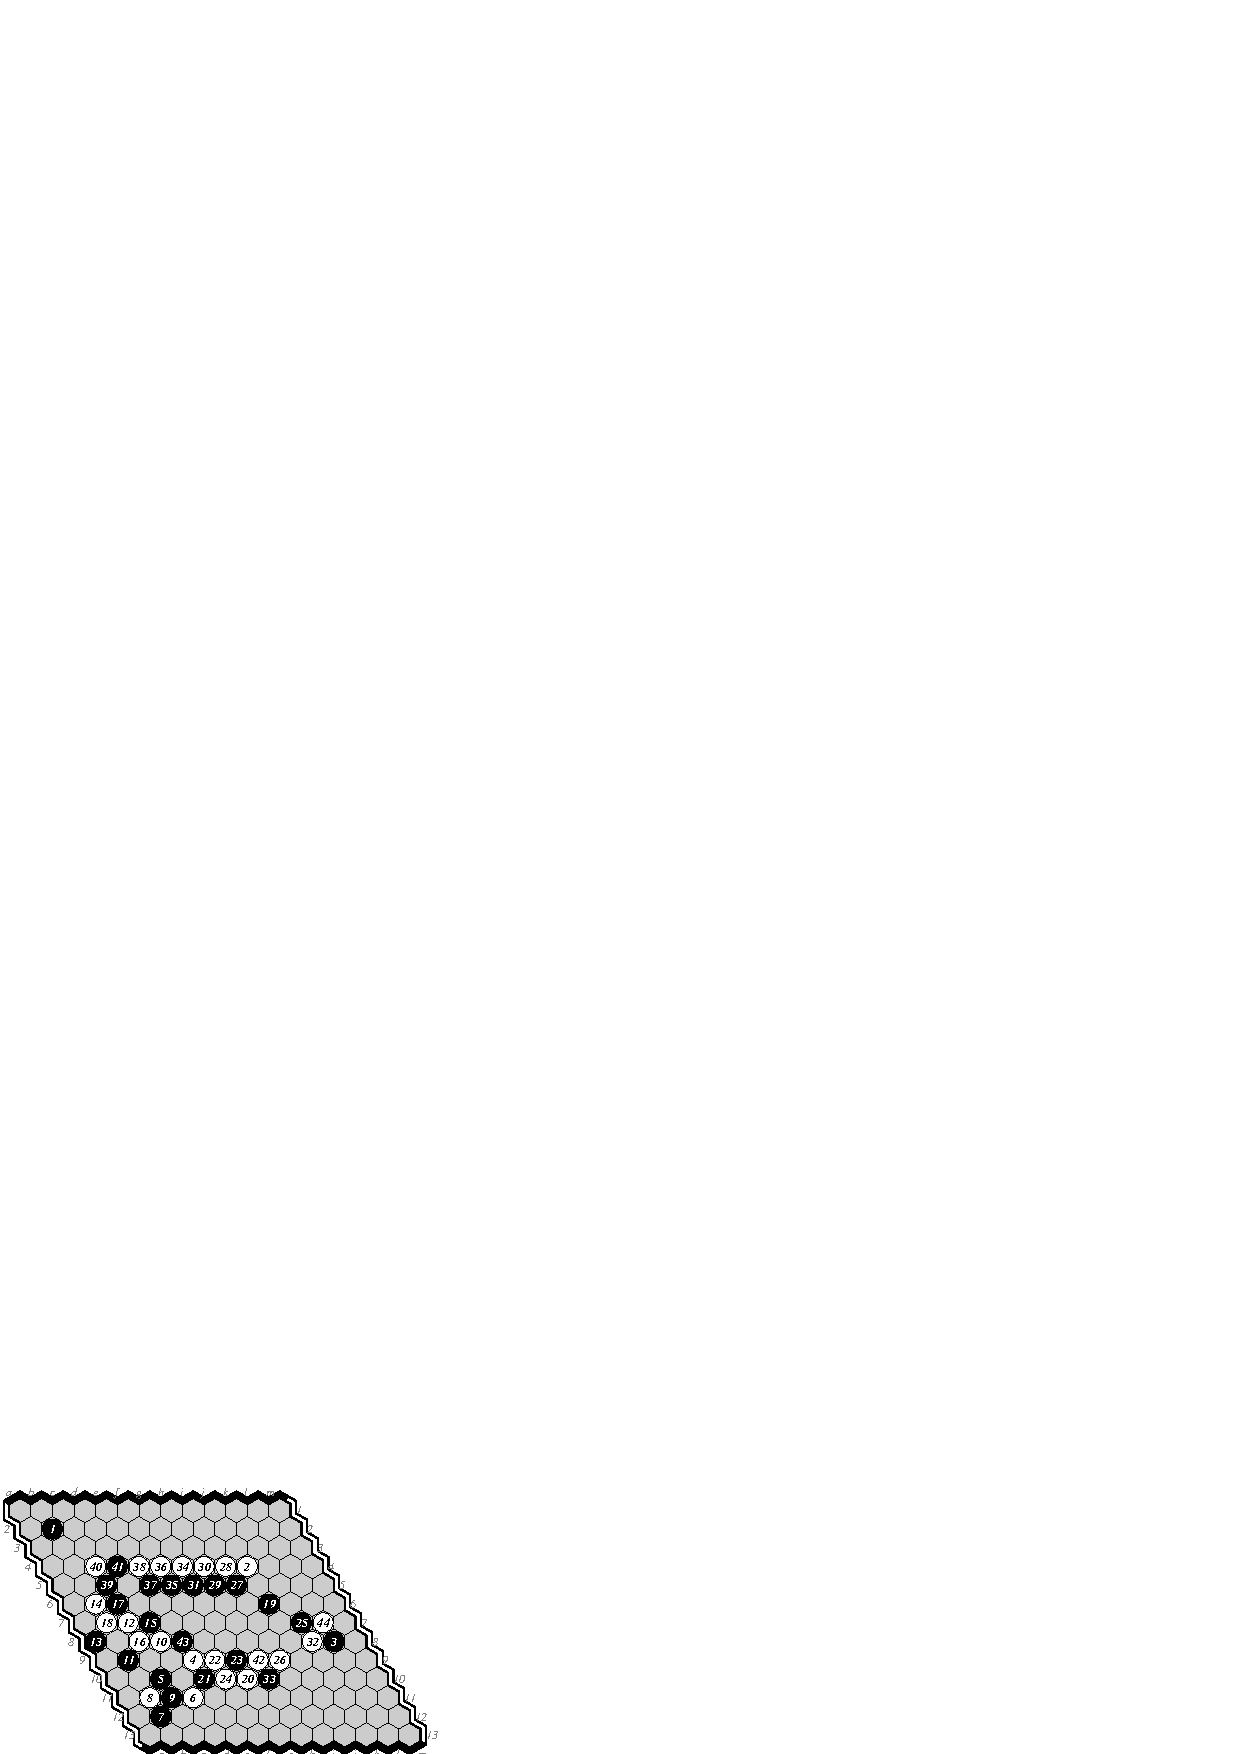
\includegraphics[width=.58\columnwidth]{pix/04-m-e}
\vspace*{.2cm}

\noindent\hfill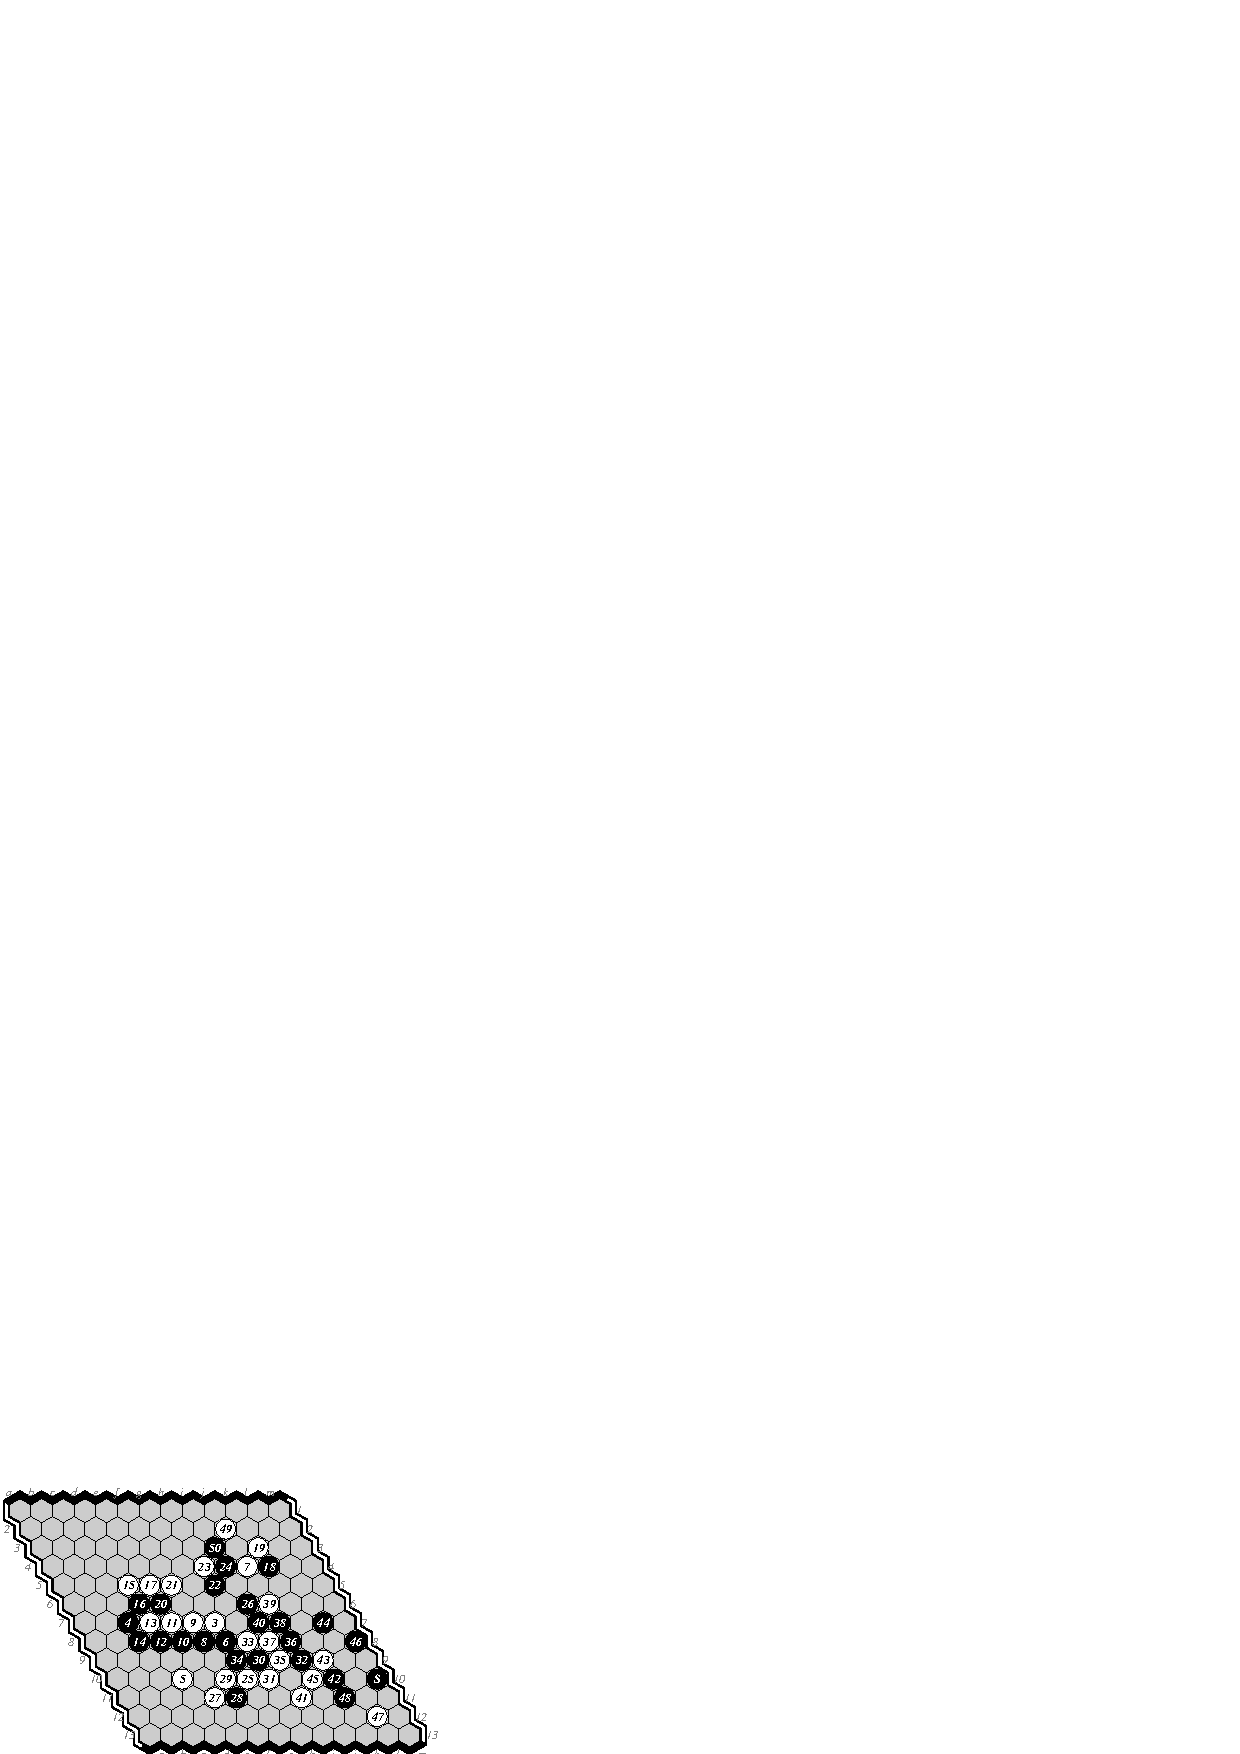
\includegraphics[width=.58\columnwidth]{pix/05-e-m}\hfill\ 
\caption{13$\times$13 Games 1-5. E-M 0-1, M-E 1-0, E-M 0-1, M-E 1-0, E-M 0-1.
S indicates that move 2 was swap.}
\label{fig:13}
\end{figure}

\begin{figure}
\noindent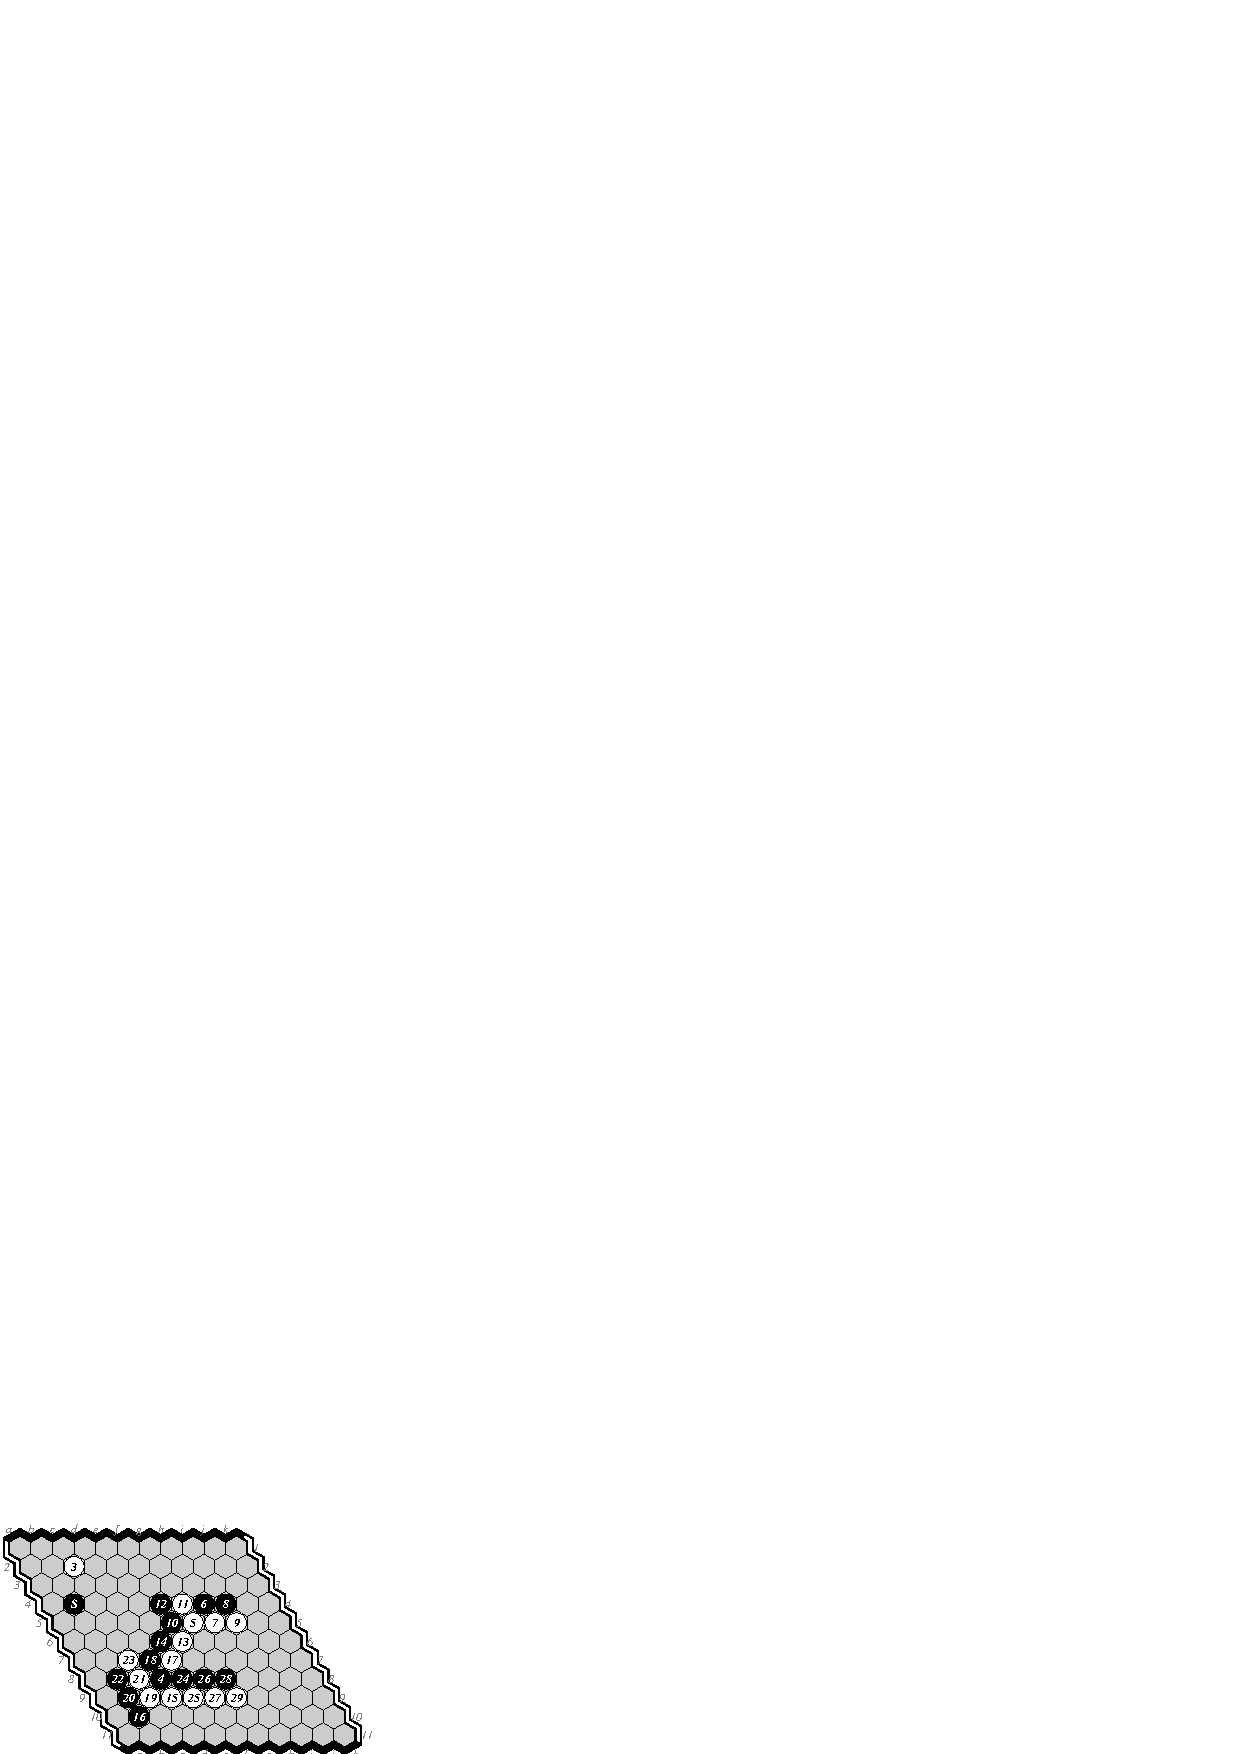
\includegraphics[width=.58\columnwidth]{pix/11-01-me}\hspace*{-.14\columnwidth}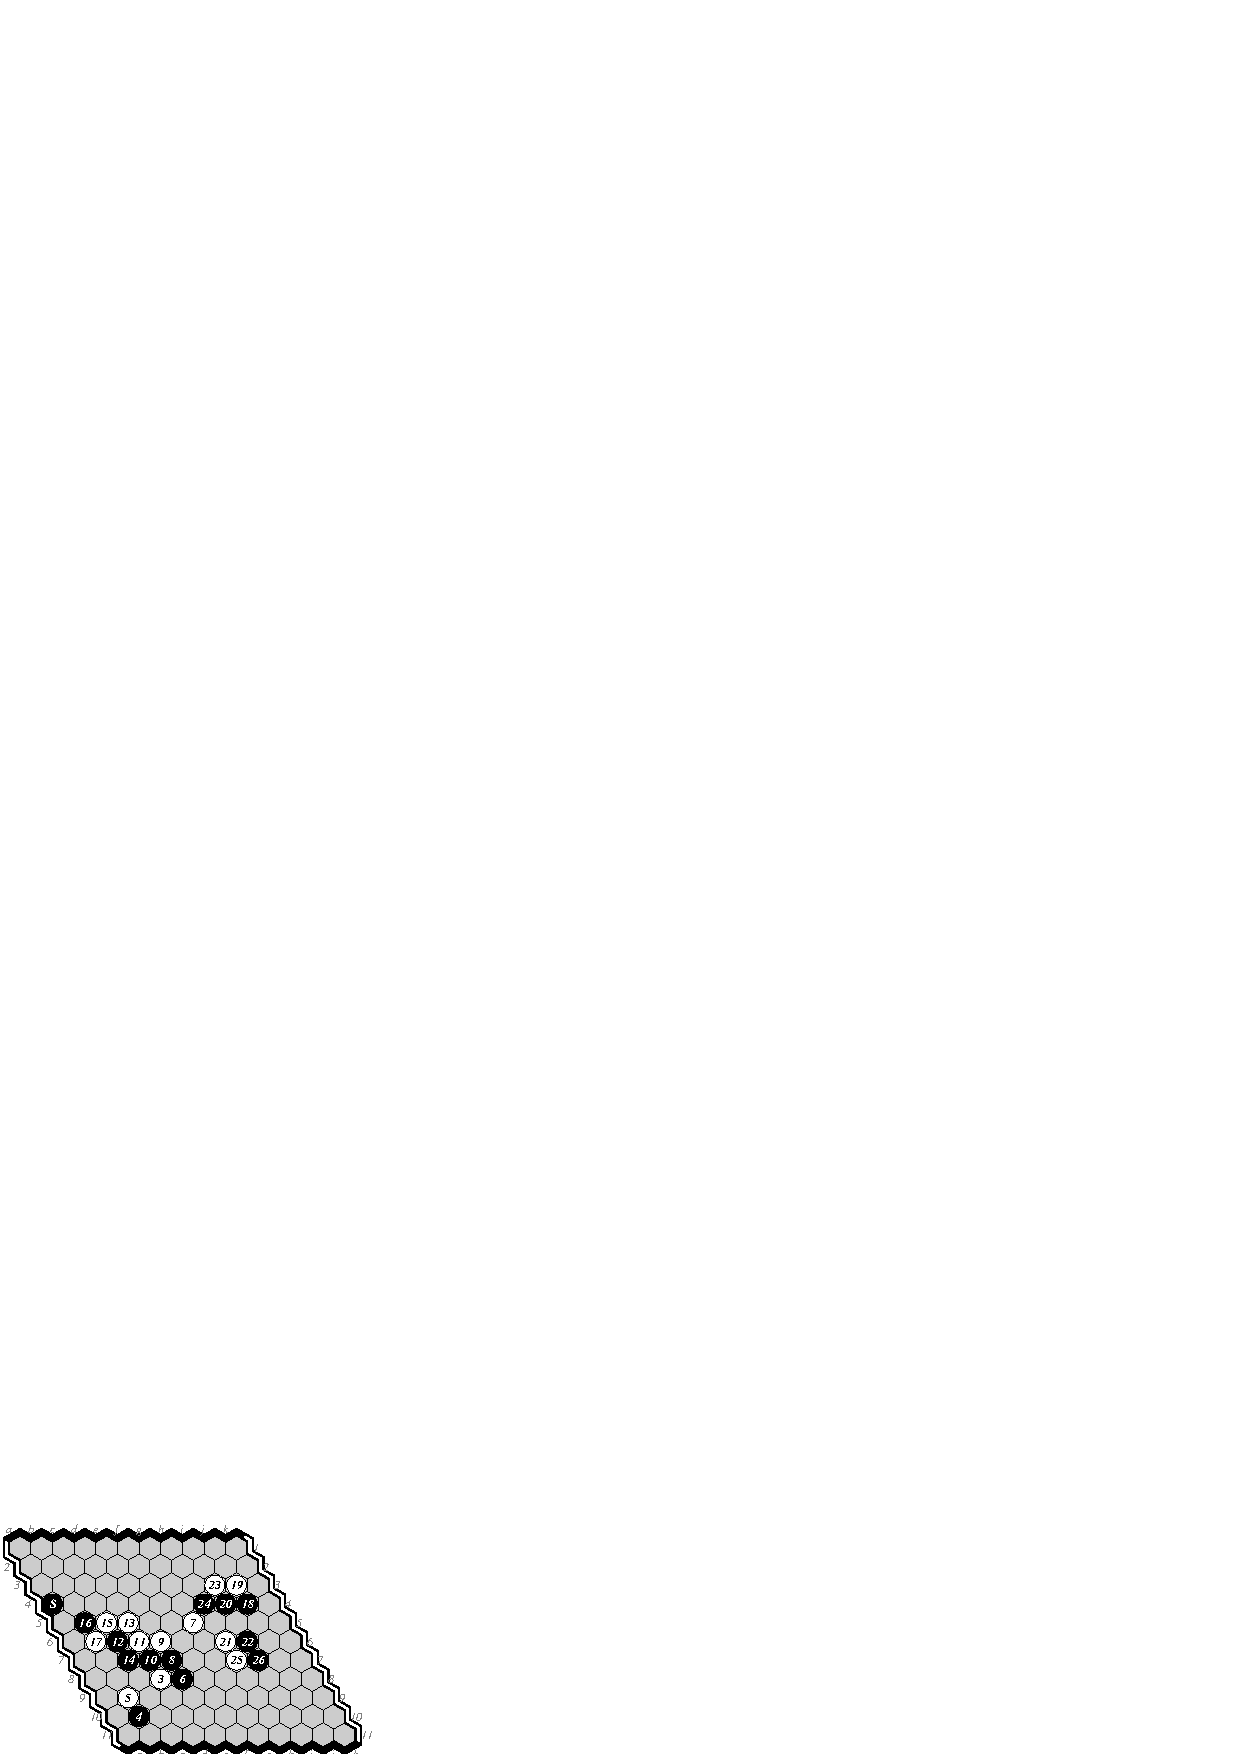
\includegraphics[width=.58\columnwidth]{pix/11-02-em}
\vspace*{.2cm}

\noindent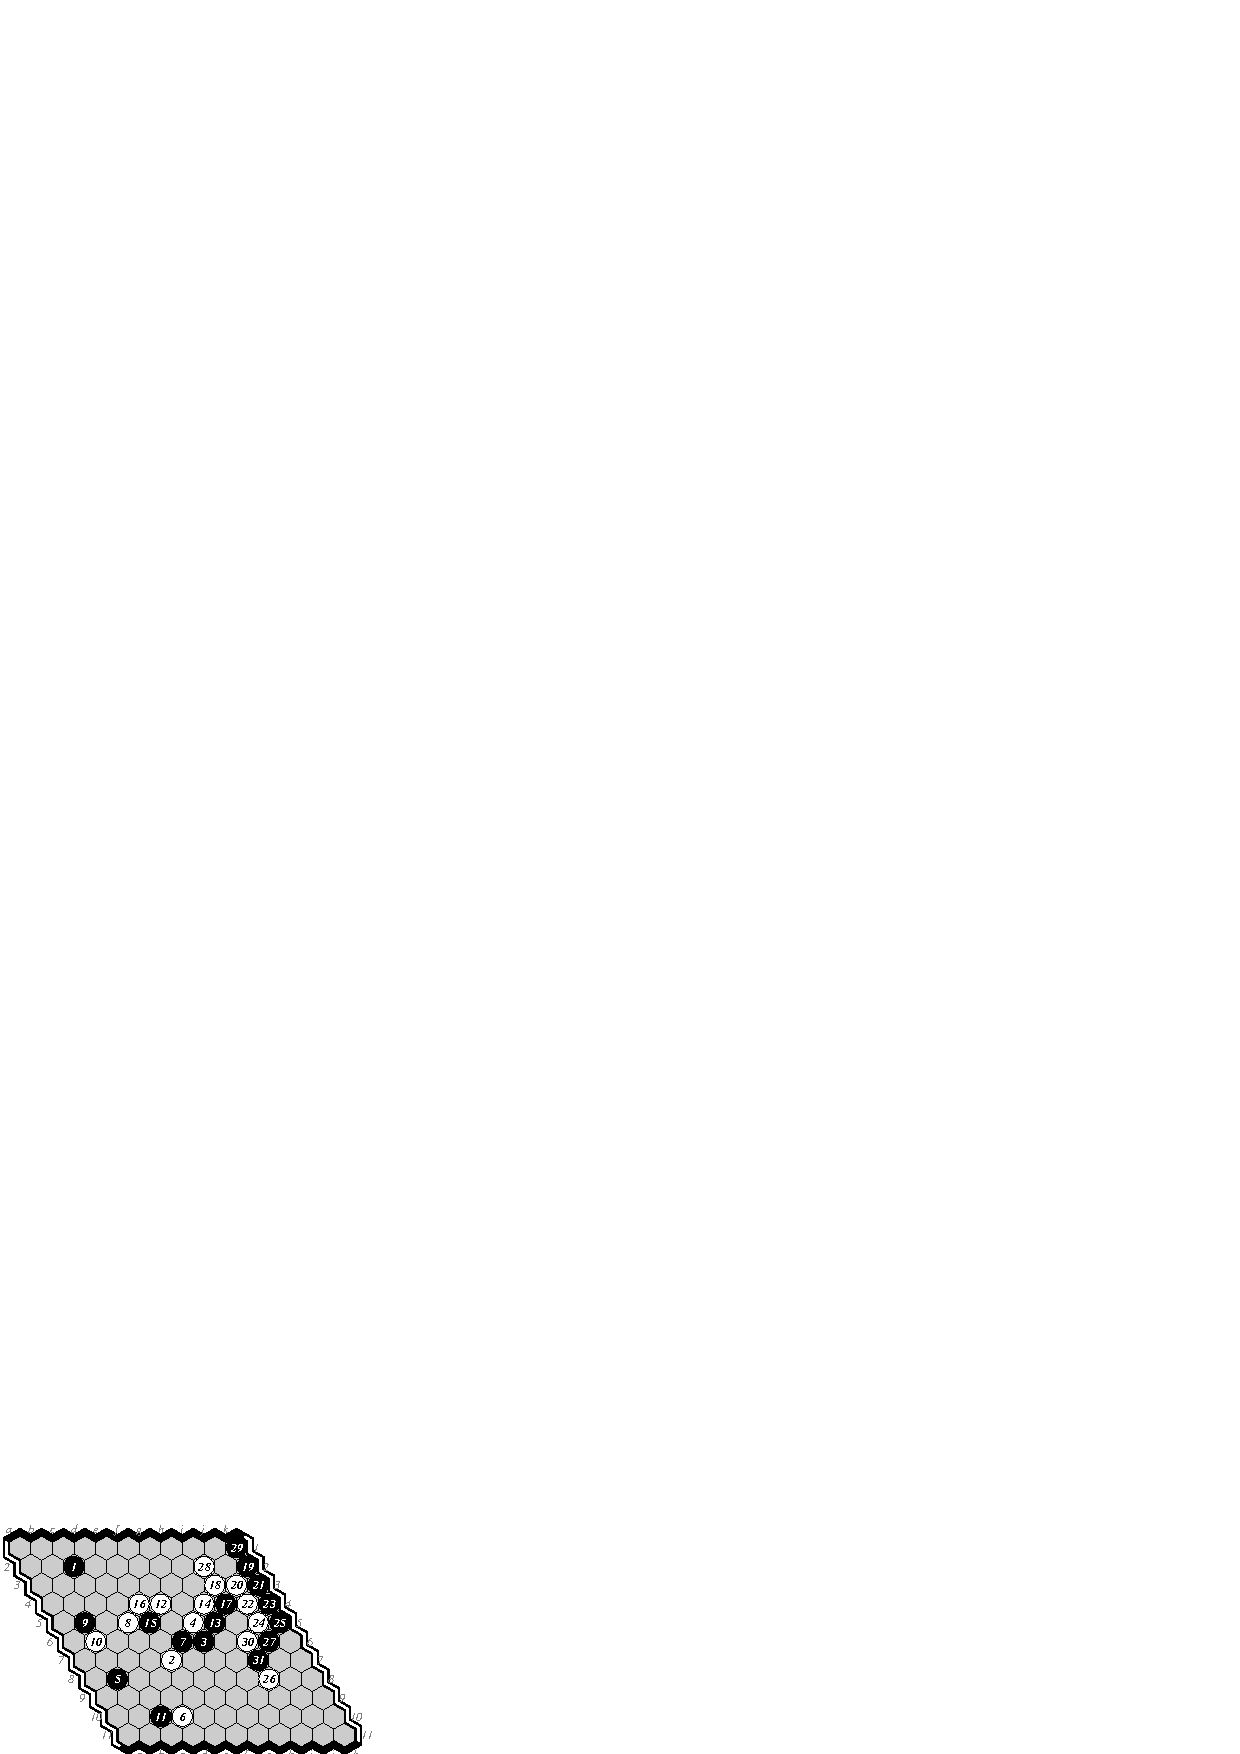
\includegraphics[width=.58\columnwidth]{pix/11-03-me}\hspace*{-.14\columnwidth}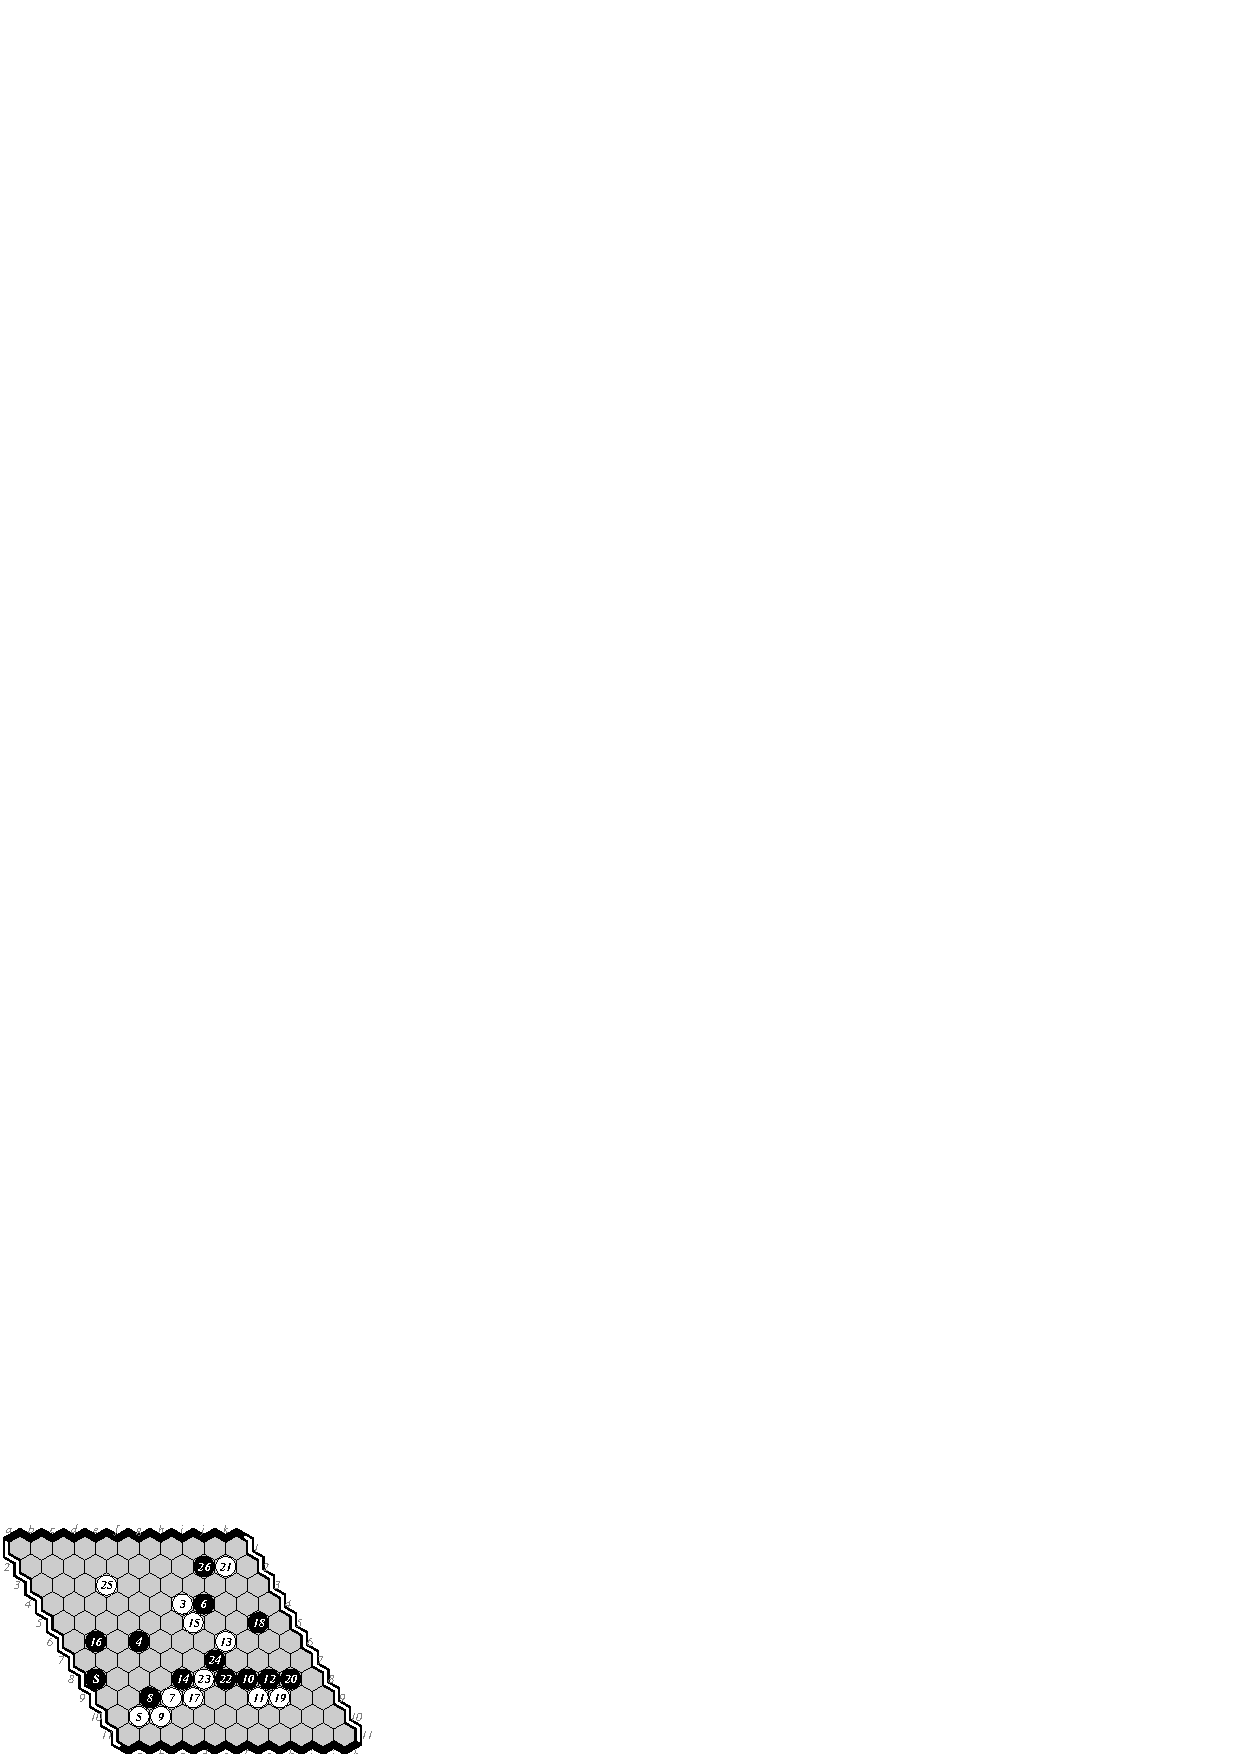
\includegraphics[width=.58\columnwidth]{pix/11-04-em}
\vspace*{.2cm}

\noindent\hfill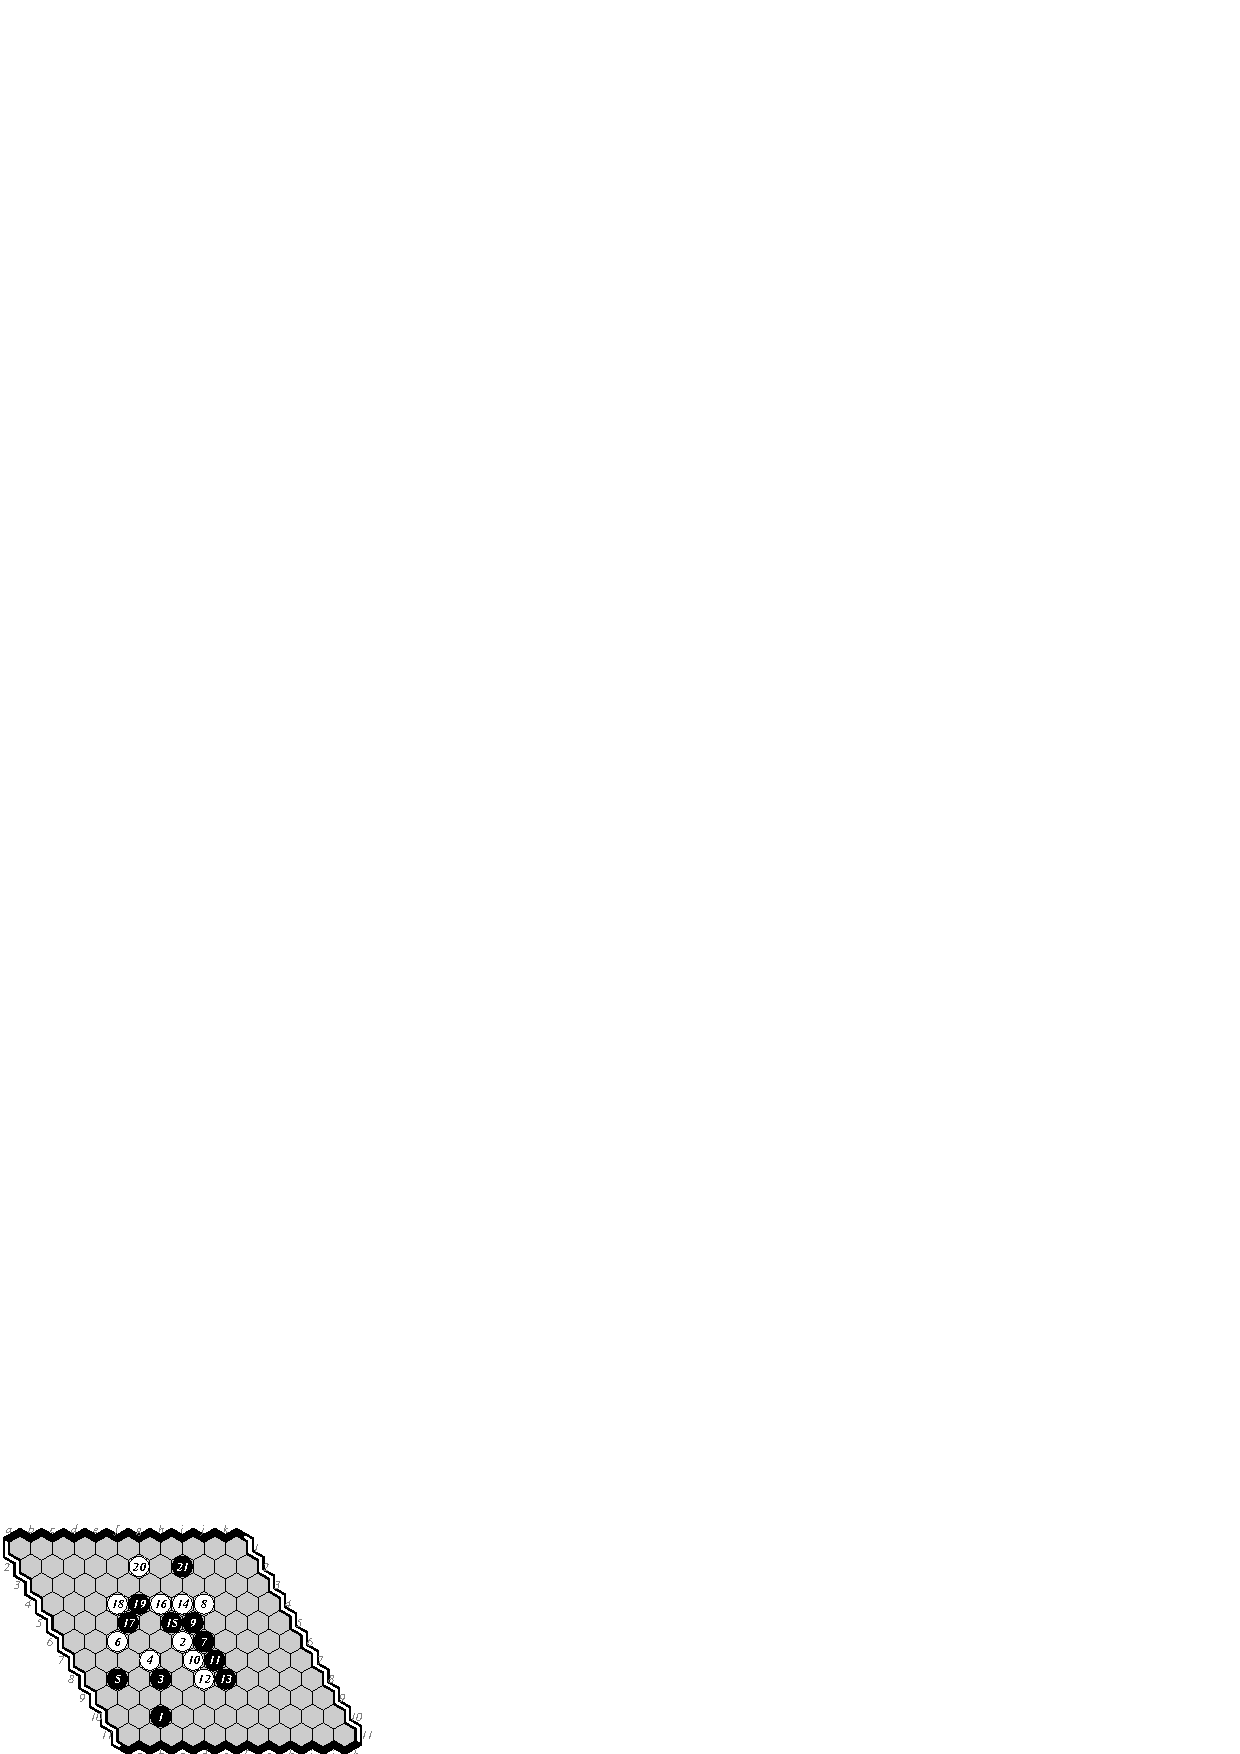
\includegraphics[width=.58\columnwidth]{pix/11-05-me}\hfill\ 
\caption{11$\times$11 Games 1-5. M-E 1-0, E-M 0-1, M-E 1-0, E-M 0-1, M-E 1-0.}
\label{fig:11}
\end{figure}

\section{Conclusions}
Using machine learning ideas inspired by AlphaGo,
both programs improved significantly this year.
\Mt{} is especially strong on 11$\times$11: Move 5 in Game 5 reminds
us of Move 37 in Game 2 of the AlphaGo-Lee Sedol match:
we have never seen this move before, 
but by the end of the game its utility is clear.
Hopefully we will see similar moves next year
on the 13$\times$13 and 19$\times$19 boards.

\section*{Acknowledgements}
We thank the NSERC Discovery Grant Program for research funding.
\bibliographystyle{plain}
\bibliography{rpt}
\end{document}
